\chapter{Použité webové technológie}
\section{Databáza}
V tejto sekcii sa čitateľ zoznámi s NoSQL databázou MongoDB a knižnicou Mongoose.

\subsection{MongoDB}
\label{mongodb}
TODO

\subsection{Mongoose}
TODO

\section{TypeScript}
\label{typescript}
TODO

\section{Frontend}
TODO

\subsection{HTML}
TODO

\subsection{CSS}
TODO

\subsection{Vue.js}
Vue.js\cite{vue-guide} patrí medzi najpopulárnejšie nástroje pre tvorbu Single Page Aplikácií. Je výkonný, rýchly a minimalistický. Veľkou výhodou je, že patrí medzi progresívne frameworky, našu aplikáciu vieme rozdeliť na viacero častí, ktoré môžu byť samostatne vyvíjané. Stal sa jedným z obľúbených kvôli jeho jednoduchosti. Má veľmi prehľadnú a pestrú dokumentáciu v anglickom aj čínskom jazyku.

Framework bol vytvorený Evanom Youom, ktorý pracoval v Googlu a Meteoru. V Googlu začal používať AngularJS, ktorým sa inšpiroval, ale tento framework mu nevyhovoval kvôli jeho striktnému písaniu kódu. Jeho motiváciou bolo vziať najlepšie vlastnosti Angularu a vytvoriť z nich nástroj, ktorý mu zjednoduší a zefektívni prácu.

Dizajn Vue.js sa inšpiroval MVVM\footnote{Model-View-ViewModel} architektúrou. Zameriava sa na vrstvu pohľadu. Spája pohľad a model cez dvojstrannú väzbu (anglicky two-way binding), ako je vidieť na obrázku \ref{pic:mvvm}. Ostatné funkcionality SPA, ako smerovanie a store môžu byť doplnené cez pomocné knižnice.
    \begin{figure}[!hbt]
        \centering
        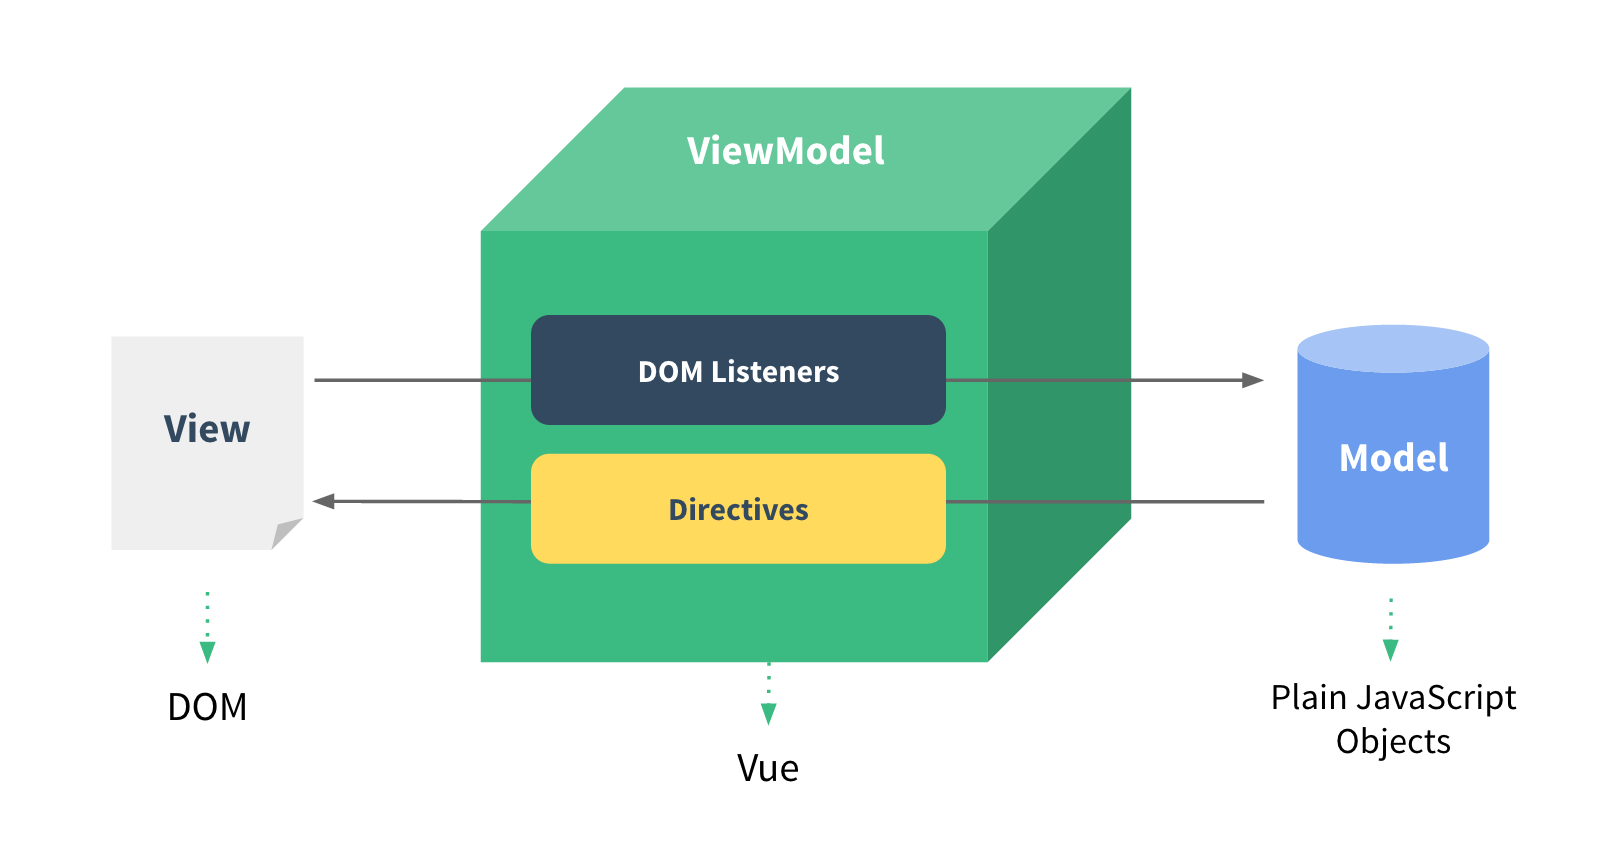
\includegraphics[scale=0.2]{obrazky/mvvm.png}
        \caption{Znázornenie úlohy Vue.js v MVVM architektúre \cite{vue-guide}.}
        \label{pic:mvvm}
    \end{figure}

\subsection*{Inštalácia}
Vue.js bol vytvorený aby bol ľahko osvojiteľný a a použiteľný. Môže byť začlenený do projektu viacerými spôsobmi. 

Štyri hlavné spôsoby sú nasledovné:
    \begin{itemize}
        \item Importovanie balíčka do HTML stránky cez CDN:
        \begin{verbatim}<script src="https://unpkg.com/vue@next"></script>\end{verbatim}
        \item Stiahnutie JavaScriptových súborov a importovanie ich rovnakým spôsobom ako u CDN
        \item Inštalácia cez správcu balíčkov npm
        \item Použitie oficiálneho CLI pre zkonštruovanie projektu
    \end{itemize}
    
\subsection*{Komponenty}
Komponenty hrajú vo Vue.js veľmi dôležitú rolu, umožňujú tvorbu vysoko škálovateľnej aplikácie, ktorá je poskladaná z malých a znovupoužiteľných častí. Môžeme mať komponenty napríklad pre hlavičku, bočný panel, obsah, ktoré môžu obsahovať ďalšie komponenty pre zoznam prezentácií, výpis detailu prezentácie. Výsledkom rozdelenia do jednotlivých častí je ľahko udržateľný a prehľadný zdrojový kód. Komponenty tvarujú hierarchiu vnoreného stromu, ktorý je znázornený na obrázku \ref{pic:components}. Tento strom reprezentuje aplikačné rozhranie.
    \begin{figure}[!hbt]
        \centering
        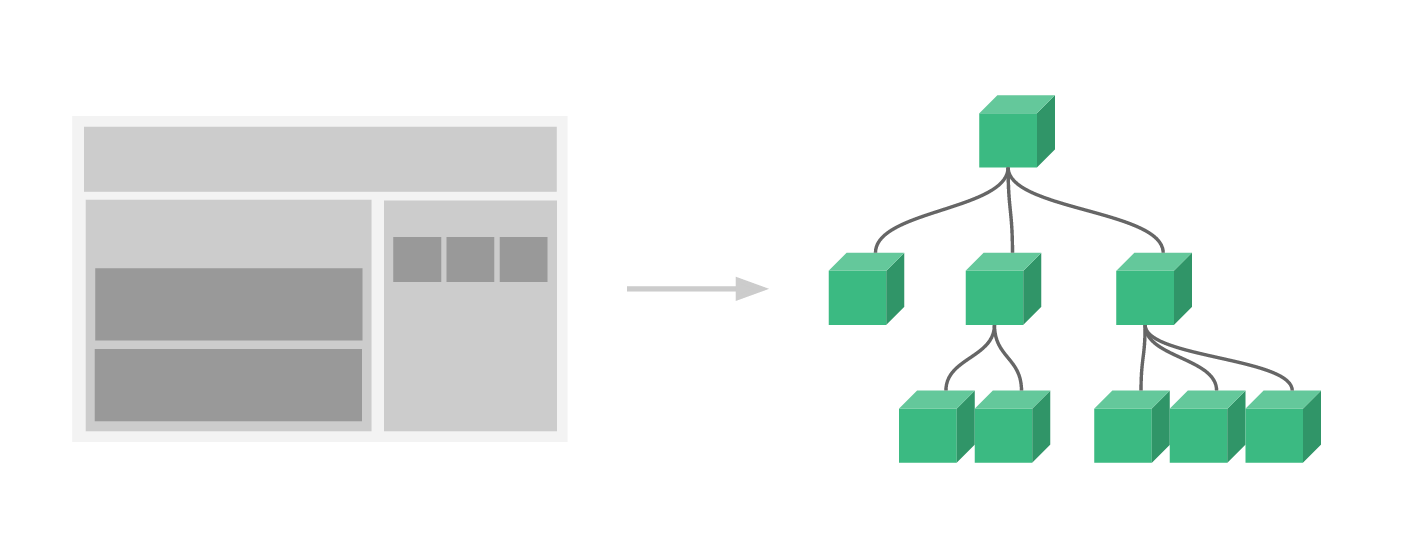
\includegraphics[scale=0.25]{obrazky/components.png}
        \caption{Znázornenie komponentov ako vnorený strom\cite{vue-guide}.}
        \label{pic:components}
    \end{figure}
    
\subsection*{Registrovanie komponentov}
Existujú dva postupy registrovania jednotlivých komponentov: \textit{lokálne} a \textit{globálne}. Lokálne komponenty je potrebné pred každým použitím importovať, narozdiel od globálnych, ktoré stačí zaregistrovať raz a môžu byť použité v šablóne hociktorej komponenty. 

Typický príklad pre globálnu komponentu je dizajnový prvok ako napríklad animácia pri načítaní údajov, takzvaný spinner. Tento typ animácie sa používa pri každom načítaní údajov, na viacerých miestach v aplikácii. Aby sme ho nemuseli po každom importovať stačí keď si ho raz globálne zaregistrujeme a môžme ho voľne používať. 

Príklad lokálnej komponenty je formulár pre registrovanie užívateľa, ktorý sa pravdepodobne použije iba raz a nepotrebujeme ho mať dostupný v celej aplikácii.

\subsection*{Komunikácia medzi komponentami}
Komponenty začnú byť viac užitočné pri vymieňaní údajov medzi sebou. Štandardne, každá jedna je izolovaná, čo znamená, že nemá prístup k rodičovským údajom. Majme komponentu pre stručný výpis informácií o prezentácii, po kliknutí na ňu sa zobrazí ďalšia komponenta s detailným výpisom. Pri tomto príklade potrebujeme predať informácie o prezentácii z jednej komponenty na druhú. Na komunikáciu medzi rodičom a potomkom sa používa \texttt{props} a metóda \texttt{\$emit}.

Props sú atribúty, ktorým vieme nastaviť hodnoty. Slúžia na predanie údajov z rodiča na potomka. Po nadobudnutí hodnoty sa z nich stanú premenné použiteľné v komponente. Počet props nie je obmedzený a prijíma ľubovolný typ údajov.

Metóda \$emit slúži na komunikáciu opačným smerom. Pomocou tejto metódy vieme vytvoriť vlastnú udalosť, ktorú rodič môže odpočúvať. Majme komponentu potomka v ktorej sa nachádza tlačítko. Kliknutím na tlačítko sa zavolá metóda \$emit do ktorej sa predá meno udalosti a ľubovolný údaj. Rodičovská komponenta môže odchytiť túto udalosť a reagovať na ňu. Vysielanie udalostí je užitočné keď máme viacero potomkov s rovnakou logikou, týmto spôsobom nemusia všetky tieto komponenty obsahovať tú istú logiku, stačí keď bude implementovaná iba v rodičovskej komponente a pristúpi sa k nej cez \$emit.

\subsection*{Životný cyklus komponenty}
Vo Vue.js každá komponenta je samostatná Vue inštancia\footnote{Jeden konkrétny exemplár triedy} a každá inštancia má svoj životný cyklus. Životný cyklus komponenty sa skladá z niekoľkých krokov, ako napríklad jej vytvorenie, pripevnenie inštancie k DOM\footnote{Objektový model HTML dokumentu}, aktualizácia DOM-u pri zmene údajov alebo jej zrušenie. Vývojári majú pri každom kroku možnosť pridania vlastného kódu cez funkcie \texttt{lifecycle hooks}. Medzi najpoužívanejšie patria:
    \begin{itemize}
        \item\texttt{beforeCreated} - Volá sa hneď po inicializácii inštancie, ktorá zatiaľ nič neobsahuje.
        \item\texttt{created} - Pri tomto kroku sa dokončilo nastavenie pozorovania dát, computed premenných, metód a udalostí. Zatiaľ nemáme prístup k DOM. Môže sa použiť pre registrovanie vlastných udalostí.
        \item\texttt{beforeMount} - Volá sa pred pripevnením DOM.
        \item\texttt{mounted} - Najpoužívanejšia funkcia lifecycle hook. Volá sa po pripevnení inštancie k DOM. V tejto funkcii už máme prístup k jednotlivým elementom v DOM. Častokrát používaná pre sťahovanie dát z API.
        \item\texttt{beforeUpdate} - Volá sa pri zmene dát. Máme prístup k existujúcemu DOM pred jeho aktualizáciou.
        \item\texttt{updated} - Funkcia volaná po znova-vykreslení DOM.
        \item\texttt{beforeUnmount} - Volá sa pred odpojením inštancie od DOM-u.
        \item\texttt{unmounted} - Po tomto kroku je inštancia kompletne odpojená, taktiež jej potomky a udalosti. Používaná pre odpojenie vlastných udalostí.
    \end{itemize}

Pri použití Composition API, o ktorom si povieme viac v sekcii \ref{compositionapi}, sa tieto funkcie trochu líšia. Lifecycle hooky beforeCreated a created sú súčasťou funkcie \texttt{setup()} a pred každý hook treba pridať predponu \texttt{on}: onCreated, onMounted, atď. 

    \begin{figure}[!hbt]
        \centering
        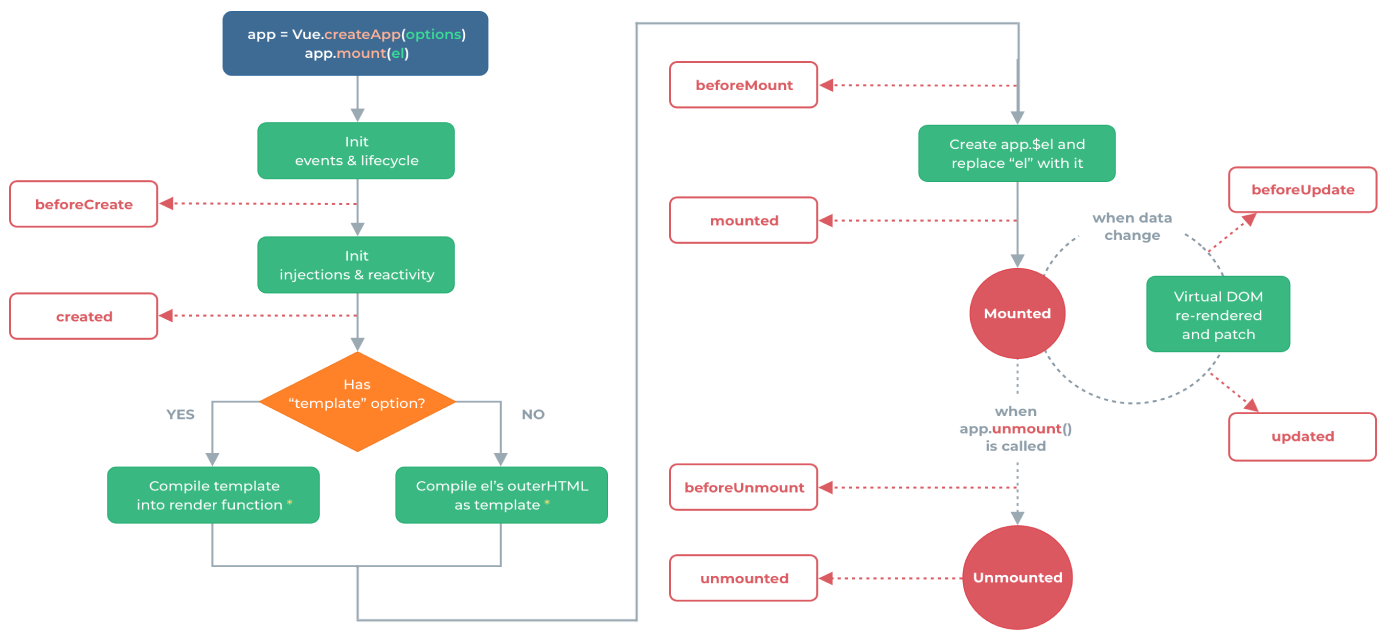
\includegraphics[scale=0.3]{obrazky/lifecycle.png}
        \caption{Graf životného cyklu komponenty\cite{vue-guide}.}
        \label{pic:components}
    \end{figure}

\subsection*{Šablóna}
Komponenta sa vykresľuje cez HTML šablónu. Okrem základnej funkcionality jazyka HTML umožňuje aj výpis statických aj dynamických hodnôt, dynamickú aktualizáciu CSS štýlov a tried, použitie podmienok na obmedzenie vykresľovania a použitie cyklov pre prechádzanie hodnôt v poli. V šablóna má vývojár prístup k premenným aj metódam. Obsah šablóny sa musí nachádzať medzi značkou \texttt{<template>}.

\subsection{Composition API}
\label{compositionapi}
TODO

\subsection{Nuxt.js}
TODO

\subsection{Reveal.js}
TODO

\subsection{Ostatné balíčky a knižnice}
TODO

\section{Backend}
TODO

\subsection{Node.js a Express.js}
\label{node}
TODO

\subsection{API}
TODO

\subsection{Ostatné balíčky a knižnice}
TODO